\section{\texorpdfstring{Event selection for the \Tau\Tau channel}{Event selection for the tau-tau channel}}
\label{sect:tauTauCuts}
In this channel events are first selected with a trigger \cite{Khachatryan:2015hwa,Chatrchyan:2012xi,Chatrchyan:2011nv}
that requires the existence of
two loosely identified, isolated \Tau candidates with \PT $>$ 35 \GeV and $|\eta|<$2.1.   

Offline , the two \Tau candidates must pass tighter identification requirements with \PT $>$ 45 \GeV and be of opposite charge.
In events with more than one \Tau\Tau pair, we only consider the pair with the tightest isolated \Tau's. 

Events with isolated extra electrons or muons of \PT $>$ 10 \GeV and $|\eta| <$ 2.4 
are rejected to suppress %the contribution of the associatiated production of \Z with vector bosons.
backgrounds from diboson decays.
The background from \Z$\rightarrow$\Tau\Tau events is reduced by rejecting events where the visible
di-\Tau invariant mass is between 55 and 85 \GeV.  Furthermore, 
low-mass Drell-Yan and QCD events are reduced by requiring the invariant mass be greater than 15 \GeV.
Loose requirements \MPT $>$ 30 \GeV and \mttwo $>$ 40 \GeV increases the rejection power against QCD multijet events.
The minimum angle $\Delta\phi$ in the transverse plane between the \ptvecmiss and any of the jets must be greater than 1. 
It should be noted the jet objects include electrons, photons, \Tau and b-tagged jets.
This requirement reduces backgrounds from QCD multijet events and \wjets events.

After applying the pre-selection described above,
additional requirements are introduced to define two search regions.
The first search region (\binone) is defined with the additional requirements for models with large mass difference ($\Delta m$) 
between charginos and neutralinos.
In this case, the \mttwo signal distribution extends beyond the 
distribution of SM backgrounds.
The second search region (\bintwo) is dedicated to models with small $\Delta m$.  
In this case the sum of two transverse mass values between \Tau and \MPT , \SumMT = $\mt(\Tau^1,\MPT) + \mt(\Tau^2,\MPT)$, 
is a good discriminator between signal and SM backgrounds. 
This variable was used previously in a similar analysis from the ATLAS experiment \cite{Aad:2014yka}.

After the pre-selection, the two signal regions (SR) are defined as:
\begin{itemize}
\item {\bf SR1}: \mttwo $>$ 90 \GeV;
\item {\bf SR2}: b-tagged jets are vetoed; \mttwo $<$ 90 \GeV; and \SumMT $>$ 250 \GeV.
\end{itemize}
The veto on b-tagged jets in SR2 is intended to reduce
the $t\bar{t}$ backgrounds, which
tend to populate the low \mttwo region.  For this purpose, jets are b-tagged
using the medium working point of the combined secondary vertex algorithm \cite{Chatrchyan:2012jua}. 

The distributions of $\mttwo$ and $\SumMT$ for data and the SM prediction
are shown in Fig.\ref{fig:comparison} before the application of the final
requirements listed above.
In the $\SumMT$ distribution, the b-tagged jets are vetoed and \mttwo $<$ 90 \GeV is also applied.
The SM predictions in Fig.~\ref{fig:comparison} 
are from Monte Carlo events, except for the
QCD prediction which is taken from same-sign di-tau data events,
after subtracting a small contribution of same-sign non-QCD events estimated from Monte Carlo events.
The data and SM predictions are in agreement within the statistical uncertainties.
The expected distributions for a SUSY signal 
corresponding to a moderate mass difference $(m_{\chione}=240\GeV,~m_{\PSGczDo}=40\GeV)$
is also shown for illustration purposes.
\begin{figure}[!Hhtb]
\centering
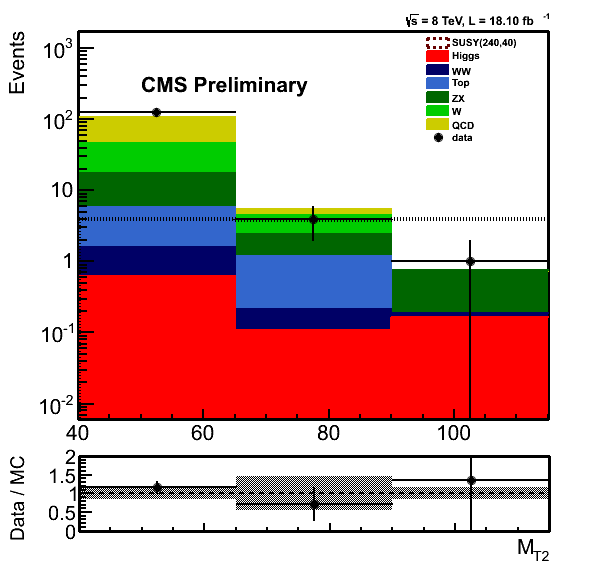
\includegraphics[angle=0,scale=0.375]{TauTauFigs/mt2.png}
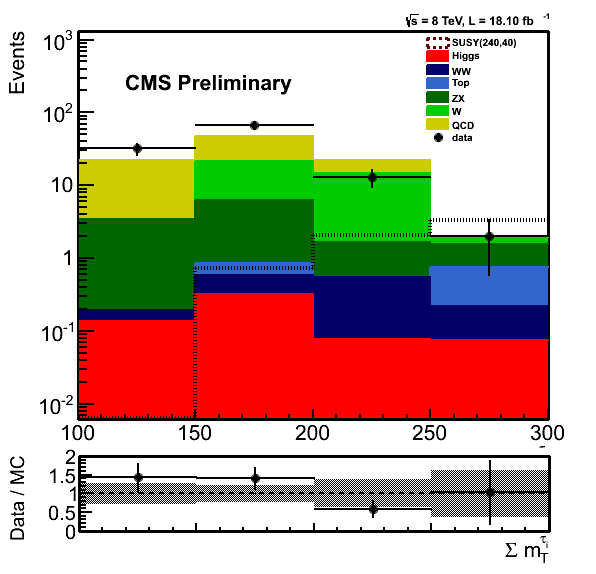
\includegraphics[angle=0,scale=0.375]{TauTauFigs/summt.png} \\ 
\caption{The distributions of \mttwo (left) and \SumMT (right) after applying all other requirements. 
The last bins of the histograms correspond to the two signal regions (\binone and \bintwo). The signal point shown here is $(m_{\chione}=240\GeV,~m_{\PSGczDo}=40\GeV)$.}
\label{fig:comparison}
\end{figure}
